\section{State of Art}

In this section we deal with the current state of the art of process control, simulation and~visualization in general and also concentrating on elementary processes in the oxygen converter used in steelmaking. There have been tremendous improvements in iron and~steelmaking processes in the past twenty years. Productivity and coke rates in the blast furnace and the ability to refine steel to demanding specifications have been improved significantly. Much of this improvement is based on the application of fundamental principles of thermodynamic and kinetic parameters which have been determined \citep{Turkdogan1999}.

\subsection{Computer-aided Mathematical Modeling and Numerical Simulation}

The motivation for using computer simulations to investigate metallurgical processes is~two-fold. First, it enables design changes to be tested before building a prototype, which naturally leads to a lower total design cost. Second, it makes it possible to investigate phenomena that cannot easily be measured or observed in the process. Even a~seemingly simple operation such as the continuous measurement of the temperature during the decarburization process is difficult due to the very high temperatures in the process and~generally harsh conditions prevailing in the steel plants \citep{Ersson2018}.

In metallurgy, simulating linear and non-linear processes that we encounter in steelmaking by creating mathematical models is of great importance. Since first attempts to use mathematical techniques for the simulation and optimization of large scale metallurgical operations \citep{Ray1973}, various numerical methods were implemented as algorithms and used to simulate phenomena in steelmaking processes. One class of such methods is~Monte Carlo, which is useful for simulating systems with many coupled degrees of~freedom such as fluids.

Modern fluid mechanics problems would be impossible to solve without use of Computational Fluid Dynamics (CFD), since the scope of analytical solutions to fundamental equations of fluid mechanics is very limited and, once a more difficult geometry is encountered, we usually have to choose a given numerical method
for obtaining a solution. CFD encompasses a wide spectrum of numerical methods used for solving complex three-dimensional (3D) and time-dependent flow problems \citep{RAPP20173}. Since early pioneering work in the metallurgical field done by \citet{Szekely1977}, the cost of performing computer simulations has decreased over the last few decades, while the available processing power has increased. Most of the processors and  processing units that are currently developed and produced have several cores that can execute instructions in parallel. Thus, the processing power available to a CFD software also depends on the capability of the software to execute in parallel. A study by \citet{Ersson2018} of the last two decades of metallurgical CFD simulations reveals huge improvements on the type of phenomena that can be explored and we will see this trend is continuing thanks to improvements in both the available processing power and the available algorithms. Therefore CFD found its way into numerous studies in steelmaking, where these methods proved useful in demonstrating the hidden and significant properties. However, its use in the steel industry may not be as integrated as in the aero and automotive industries, in~which the development of new designs is of key importance. The major difference between aero and~metallurgical industries is that the metallurgical industries almost always deal with multiphase systems at elevated temperatures and that the motivation of modeling is mainly process optimization. With a continuing development in multiphase models as~well as~in~reacting flow modeling, the continued usefulness of CFD in metallurgy remains clear.

In LD/BOF process, different chemical reactions among oxygen, slag, and molten iron in~oxygen converter, in combination with vigorous stirring process to promote slagging, dephosphorization, decarbonization, heating of molten steel, and homogenization of steel composition and temperature, determines the final properties of steel. The objective of~the~oxygen converter is to refine molten iron to crude steel through oxidization to~achieve a specified temperature and chemical composition at the end blow. Failure to do this leads to the need to reblow. The impact of oxygen jet into molten bath strongly affects the bath and promotes the three-phase flow among gas, slag, and molten steel in the bath. With the move from old rule-based systems to a model-based, real-time closed-loop control of lance movement and oxygen flow, significant drawbacks were eliminated. There have been efforts in developing accurate and efficient numerical models within CFD field to solve the jets flow in the oxygen converter. \citet{Peng1996} established the conditions of optimum nozzles of performance by deriving the system of mathematical equations to simulate the steady, quasi-one-dimensional supersonic flow through a single De Laval nozzle. \citet{Tago2003} analyzed single-nozzle and multi-nozzle lances with the help of two-dimensional simulation based on fluid dynamics and found that higher ambient temperature leads to the lower density and the higher velocity of the gas jets, but does little affect the dynamic pressure. They report that CFD proved useful method to predict the effect of the inclination angle and the number of the nozzles on the jet behavior in the top blown processes. \citet{WangW2010} developed a three-dimensional mathematical model to simulate the compressible jets flow from the top-blown lance, taking into consideration variations of fluid density, viscosity, high temperature and Mach number. They demonstrated that $k–\omega$ turbulence model is superior to the widely used $k–\epsilon$ turbulence model to calculate turbulent conditions within multiple jets. Simulation results of final computational flow field distributions of three kinds of multiple jets are shown in Fig. (\ref{o:m1}).

\begin{figure}[h!tbp]
	\centering
	\subfloat[Velocity magnitude (m/s)]{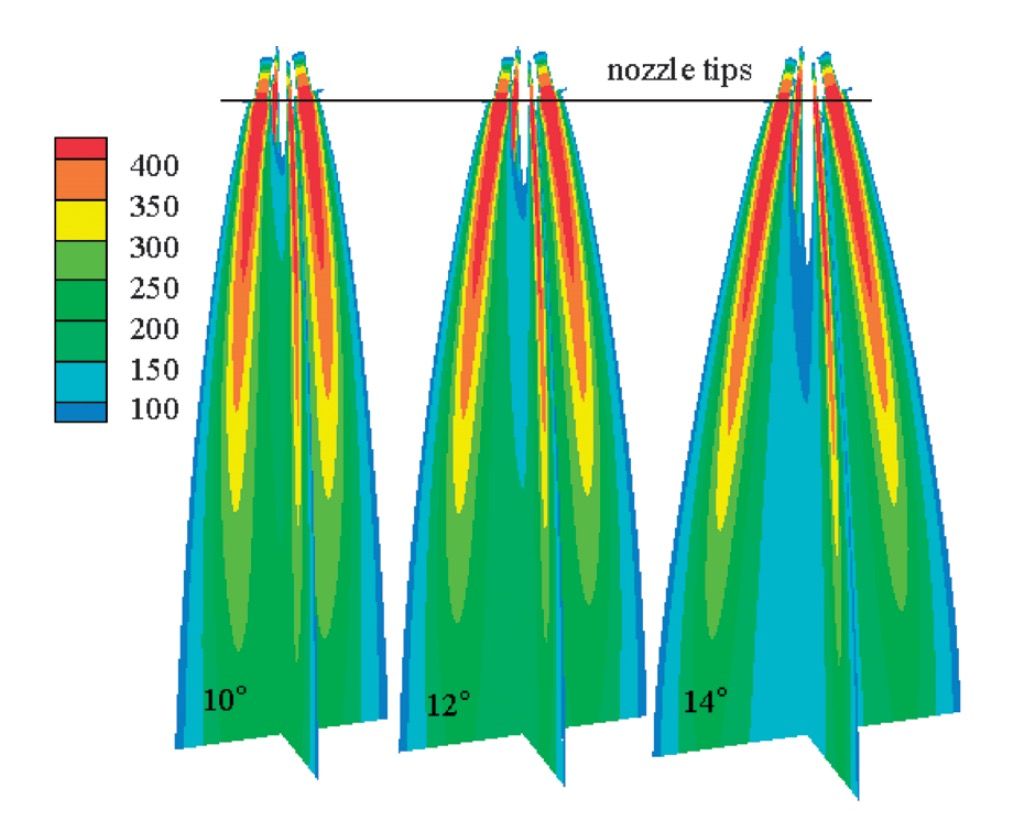
\includegraphics[width=0.6\textwidth]{cfd-velocity-magnitude.jpg}\label{fig:m1}}
	\hfill
	\subfloat[Total temperature (K)]{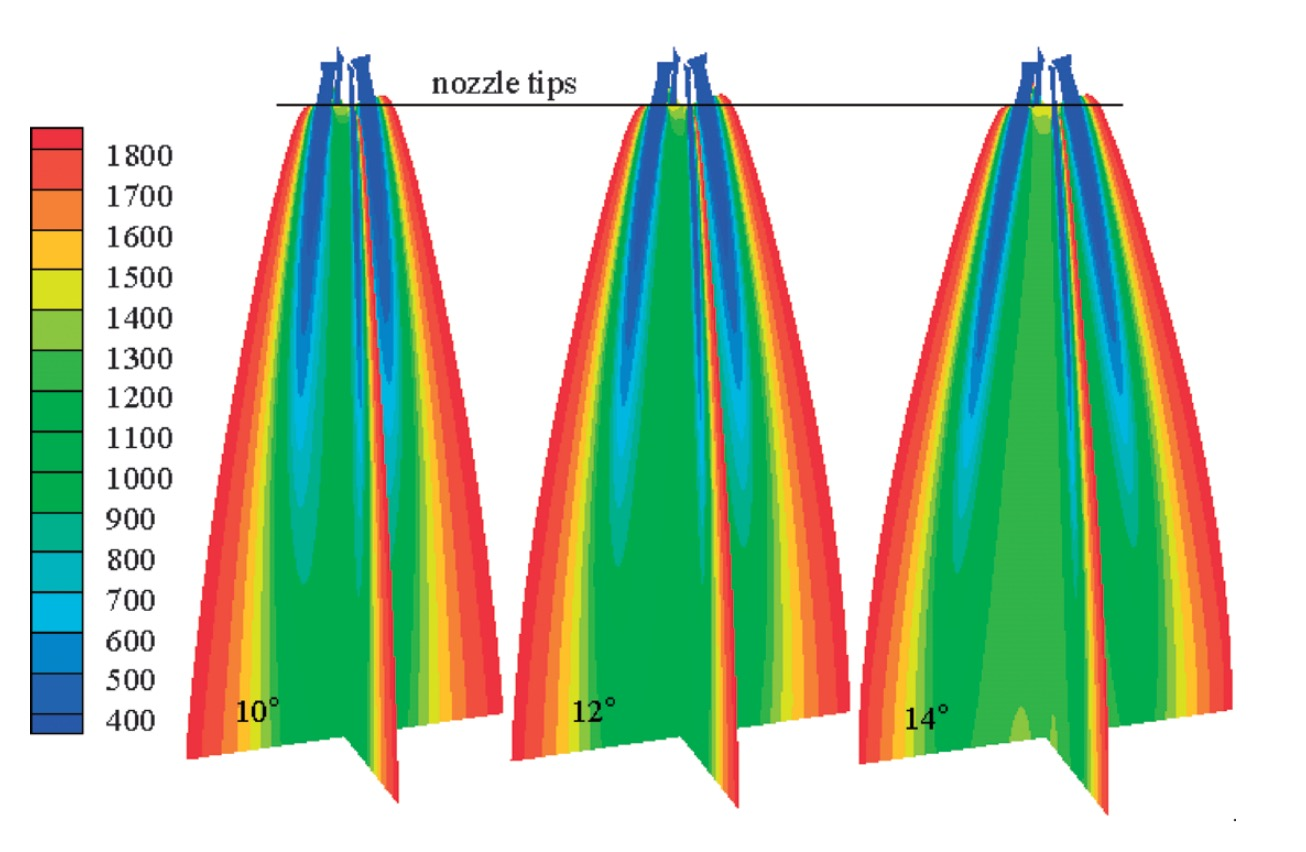
\includegraphics[width=0.7\textwidth]{cfd-total-temperature.jpg}\label{fig:m2}}
	\caption{Simulating results of velocity magnitude and total temperature field distributions of the three kinds of multiple jets: (a) velocity magnitude (m/s) and (b) total temperature (K) \citep{WangW2010}.}
	\label{o:m1}
\end{figure}

CFD models have been also used in developing deeper understanding of the decarburization processes in steelmaking. However, these processes are highly complex with large variations in time and length, and therefore it makes the systems extremely demanding to simulate. \citet{Ersson2018} reviewed latest research on the subject from 1998 until 2016 and found out that, even though several reports have been published discussing research about modeling parts of the decarburization processes numerically, no models have been presented that can handle the entire complexity of the processes. Many authors had simplified the system in existing models in order to achieve an understanding of particular phenomena rather than of the entire process.

Another important part of the oxygen steelmaking process is keeping the usual balance of~80\% hot metal and 20\% scrap during charging to regulate the temperature of steel in the vessel. To define the charge conditions and oxygen blowing requirements to achieve the temperature and chemical composition, mathematical and thermodynamic models have been developed \citep{Kacur2019,Sprava2018}. Reactions that take place in~LD process can vary significantly from heat to heat, while not many variables involved are not accurately known. Therefore, it is necessary to take into account the uncertainty affecting the whole process reactions. To correct the differences between the theoretical predictions of the process models and the real results, \citet{Bouhouche2012} introduced a random quantity term into their models and improved the prediction model with the use of Support Vector Regression and Monte Carlo Simulation methods in combination. Most of the control schemes rely on an accurate system model. However, as these systems become more complex, writing down the dynamics from the first principles is extremely challenging. In such cases, neural networks are used to approximate the dynamics directly using system data. In this context, neural networks can be thought of as a generalization of linear regression for non-linear dynamics. At the Institute of Control and Informatization of Production Processes at BERG Faculty (TUKE), team around \citet{Sprava2018} built upon Bouhouche's work and started experimenting with machine learning in process control and its application in oxygen steelmaking, precisely in LD converter. They applied Support Vector Machines (SVM) and Support Vector Regression (SVR) to predict the final melt temperature and final carbon concentration based on dynamical data. Their work also focuses on developing innovative fractional-order mathematical models for indirect measurement of molten steel temperature and concentration of \ce{CO} and \ce{CO2}. The non-linear nature of these processes presents the opportunity to model them by using derivatives of non-integer order, which in their definition are based on the influence of past data on the present value of derivative.

In some simplified form, combinations of numerical simulations and visualizations of~steelmaking processes can be used as a educational tool in process control courses at technical universities. The aim of the online, web-based interactive simulation of basic oxygen steelmaking at steeluniversity.org shown in Fig. \ref{o:m5} is to introduce students to this process in a more fun and engaging way.

\begin{figure}[ht!]
	\centering
	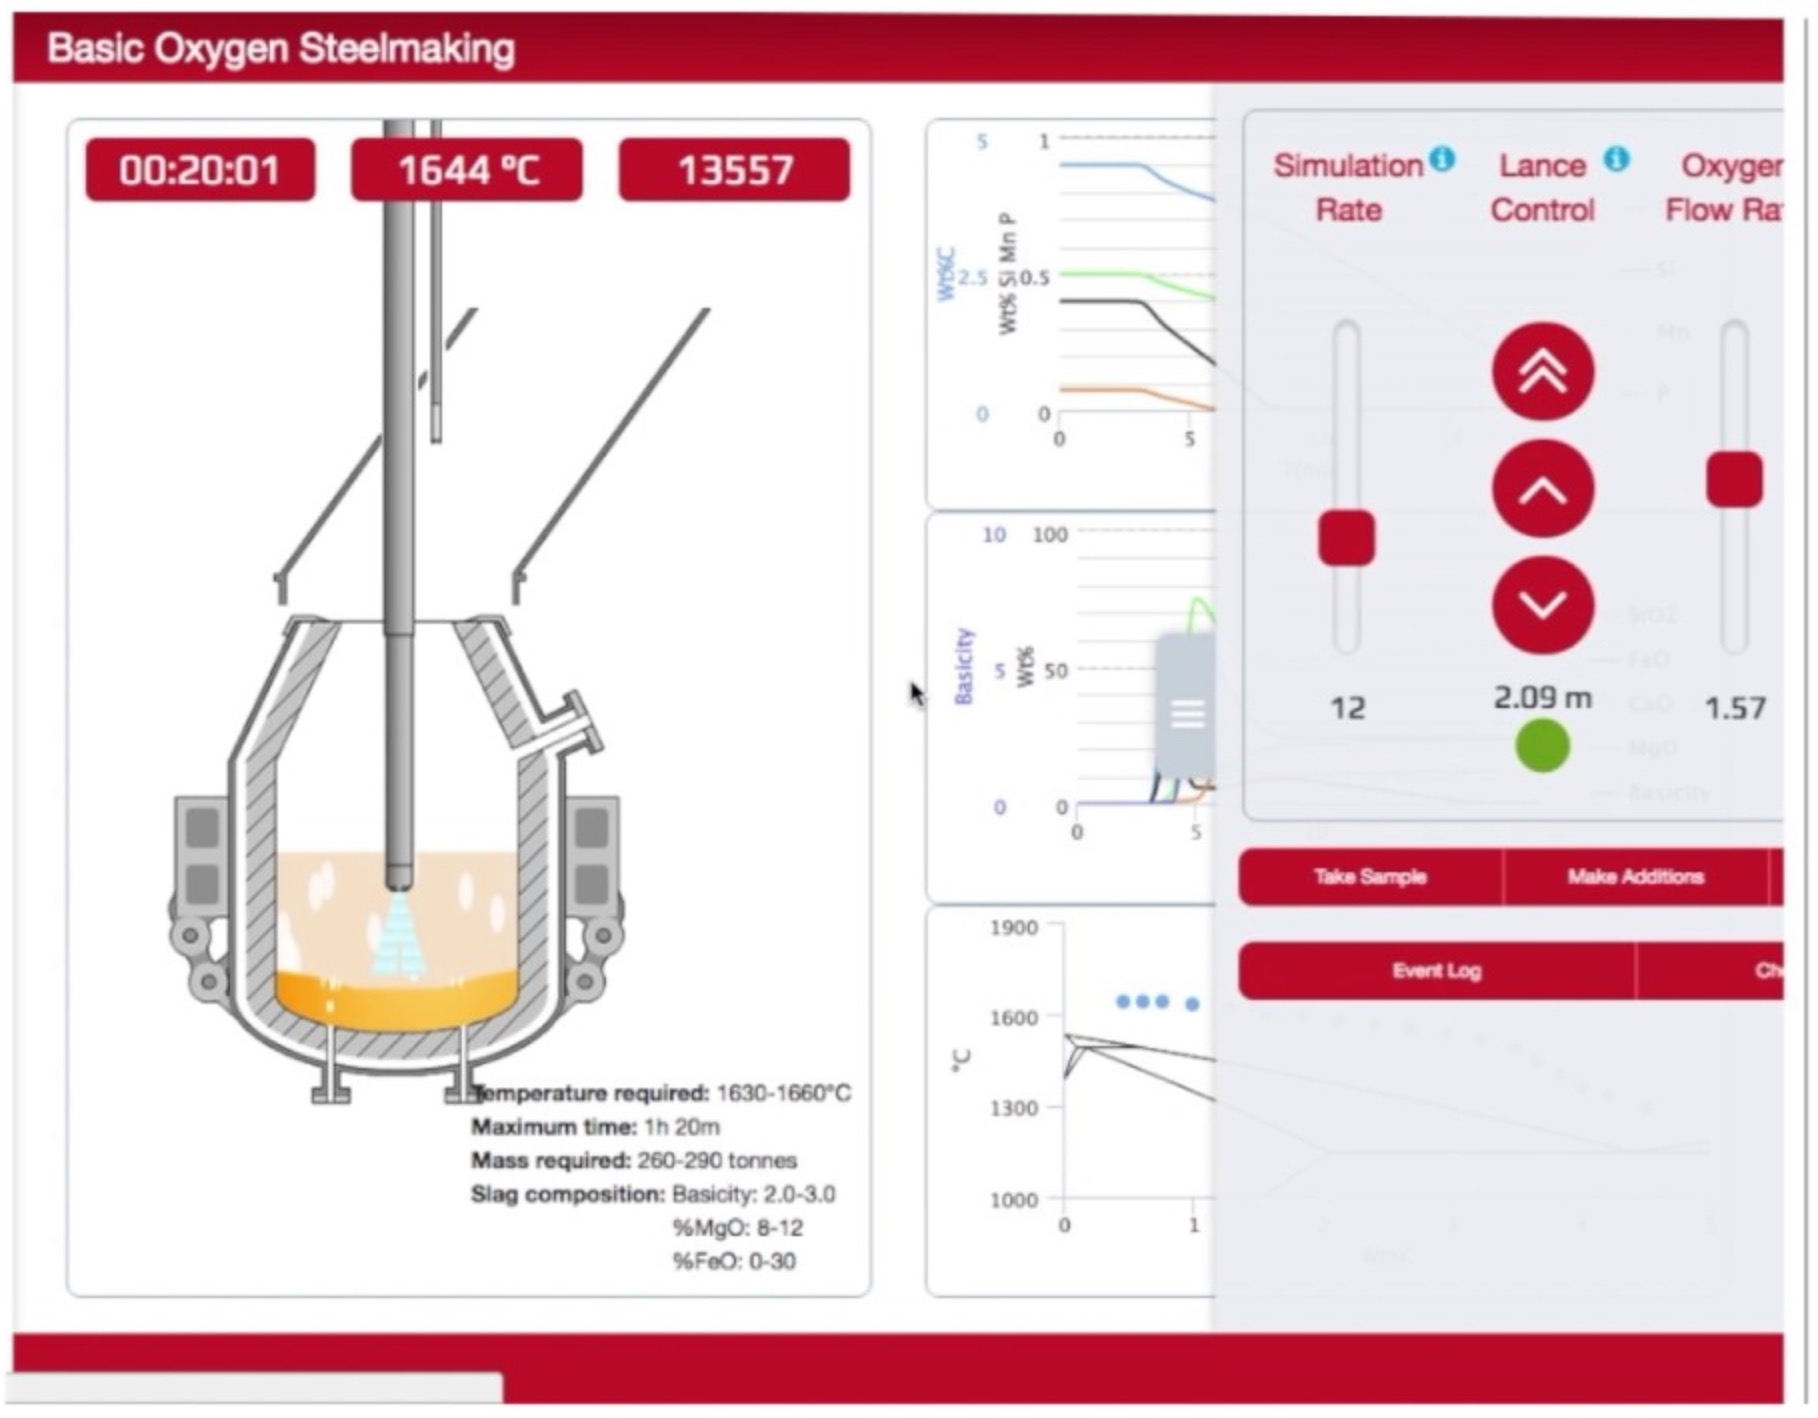
\includegraphics[width=.8\textwidth,angle=0]{steeluniversity.jpg}
	\caption{Interactive, educational simulation of basic oxygen steelmaking by steeluniversity.org.}
	\label{o:m5}
\end{figure}

\subsection{Process control}

The need for developing improved control systems has traditionally been powered by the demand for more accurate and cost efficient production. This is still a major driving force but environmental issues do also have a profound influence on this development today \citep{Widlund1998}.

The main objective of controlling oxygen converter steelmaking is to obtain prescribed parameters for the steel when it is tapped from the furnace, including weight, temperature, and each element content. In practical steelmaking process, the criterion whether the molten steel is acceptable or not is often decided by the endpoint carbon content and~temperature \citep{Wang2010}.

Generally, the LD/BOF steelmaking process with sub-lance system can be divided into two stages: static control and dynamic control. Static models include oxygen supplying model, slaging model and bottom blowing model; dynamic models include decarburization speed model, molten steel warming model and the model for the amount of coolant. \citep{Wang2010}.

The fast dynamics of the LD converter steelmaking process or the BOF process, as~it~is~commonly known, often makes it a challenge to obtain stable blowing conditions and to~achieve the required steel composition and temperature simultaneously at the end point. For this reason, process control becomes very necessary and attempts had started as early as in the 1970s \citep{Fritz2005}. Out of the originally very simple LD process have grown the modern process-controlled and automated production systems that enable present-day adaptations to meet today's economic and ecological demands \citep{Sarkar2015}. The non-linear nature of chemical and thermodynamical processes in basic oxygen steelmaking also amassed interest in developing new mathematical models based on fractional-order calculus.

\subsection{Visualization and Virtual Reality}
\label{subsection:2.4}

Scientific visualization is the use of computer graphics to create visual images that aid in~the understanding of complex numerical representations of scientific concepts or results. Computational fluid dynamics (CFD) based numerical simulations often output massive amounts of data. These simulations often contain high-dimensional data in~a~three-dimensional volume. The display of phenomena associated with this data may involve complex three-dimensional structures.

Non-immersive interactive visualization systems implemented for the conventional desktop and mouse are effective for moderately complex problems. \citet{Kealy2006} defines mouse-based interactivity type of virtual reality as "virtual realia". \citet{Milgram1994} puts forward and idea of "virtuality continuum" in his Extent of Presence Metaphor, where he states that virtual realia type of desktop virtual reality visualization is essentially a "window-on-the-world" with a fixed monoscopic viewpoint; changes in the viewer’s head position do not result in different perspectives of the object.

Immersive virtual environments, by comparison, lie at the other end of the spectrum and~permit looking around an object by moving one's head position. Therefore, a fundamental difference between desktop-and-mouse virtual realia and immersive VR is that the latter is a true 3D representation that may be either viewer or object-centered while the first is exclusively viewer-centered. In other words, changes in the relative positions of~a~2D object's components result from shifts in the viewer's perspective. The same may be true for objects viewed in a three dimensional environment, whether real or virtual. However, in such an environment, an object may also appear to change shape (e.g., through foreshortening), not due to an altered position of the viewer, but because the object itself has moved to a different position. Immersive virtual reality displays aid in~the unambiguous display of these structures by providing a rich set of spatial and depth cues. Virtual reality interface concepts allow the rapid and intuitive exploration of the volume containing the data, enabling the phenomena at various places in the volume to~be~explored, as well as provide simple control of the visualization environment through interfaces integrated into the environment \citep{Bryson1996}.

Desktop-and-mouse interfaces for 3D visualizations make it difficult to specify positions in three dimensions and do not provide unambiguous display of 3D structure. Virtual reality interfaces attempt to provide the most anthropomorphic interfaces possible - that means they must be human-conforming and should be designed to allow the most natural, unambiguous way of scientific exploration. They must include two components: display and user control. Scientific visualization makes particular demands on virtual reality displays. The phenomena to be displayed in a scientific visualization application often involve delicate and detailed structure, requiring high-quality, high-resolution full-color displays. A wide field of view is often desirable, because it allows the researcher to view how detailed structures are related to larger, more global phenomena.

Historically, the early attempts at using head-mounted virtual reality technologies started with CRT-based Binocular Omni-Oriented Monitor (BOOM) created by Fakespace Systems Inc. BOOM was a stereoscopic display device with screens and optical system housed in a box that is attached to a multi-link arm. Head tracking was accomplished via sensors in the links of the arm that holds the box.

Advent of commodity-level VR hardware like HTC Vive or Oculus Touch has made this technology accessible for meaningful applications. These headset utilize lasers and photosensitive sensors (HTC Vive) or cameras (Oculus Touch) for head and hands tracking and provide six degrees of freedom (6DoF) for movement in virtual environment. By immersing the user into the simulation itself, virtual reality reveals the spatially complex structures in computational science in a way that makes them easy to understand and study. But beyond adding a 3D interface, virtual reality also means greater computational complexity \citep{Bryson1996}. The ability to provide real-time interaction can provide strong depth cues, either through allowing interactive rotations or through the use of head-tracked rendering. Applications and techniques are being developed to discern how immersive technology benefits visualization. The medical field provides an especially promising context for this development, as medical practitioners require a thorough understanding of specific 3D structures: human anatomy. Users may interact simultaneously with high resolution computed tomography (CT) scans and their corresponding, 3D anatomical structures.

Another frequently used type of immersive, interactive display technology nowadays is~projection-screen-based Cave Automatic Virtual Environment (CAVE). These systems consists of 3 to 6 large displays positioned into a room-sized cube around the observer. The walls of a CAVE are typically made up of rear-projection screens, but recently the flat panel displays are commonly used. The floor can be a downward-projection screen, a bottom projected screen or a flat panel display. The projection systems are very high-resolution due to the near distance viewing which requires very small pixel sizes to retain the illusion of reality. The user wears 3D glasses inside the CAVE to see 3D graphics generated by the CAVE. People using the CAVE can see objects apparently floating in the air, and can walk around them, getting a proper view of what they would look like in reality. This is made possible by infrared cameras. Movement of the observer in the CAVE is tracked by the sensors typically attached to the 3D glasses and the video continually adjusts to retain the viewers perspective.

Many universities and engineering companies own and use CAVE systems. Researchers can use these systems to conduct their research topic in a more effective and accessible method. Engineers have found them useful in enhancing of a product development through prototyping and testing phases.

Substantial amount of work in applying 3D visualizations and virtual reality for solving technological issues and bringing new trends into steelmaking industry is currently happening at Center for Innovation through Visualization and Simulation (CIVS) at Purdue University Northwest (located in Indiana, USA). CIVS has been globally recognized for~its integrated and application-driven approaches through state-of-the-art simulation and virtual reality visualization technologies for providing innovative solutions to solve various university research problems, industry issues, as well as education. More than 350 projects that have been completed at the center from its inception in 2014 until today provided substantial educational and economic impact, resulting in more than 40 million US dollars (more than 36.1 million € at the time of this writing) in savings for companies. In collaboration with other universities and companies from steelmaking industry, they focus on research regarding integration of virtual reality with simulation technologies and~high performance computing; application of simulation and visualization technologies to industrial processes for process design trouble-shooting and optimization to~address the issues of productivity, energy, environment, and quality; and last but not least, development of advanced learning environments in virtual reality for training and education. With funding support provided by a major AMTech grant from the U.S. Department of Commerce, they launched novel, industry-led association of steel manufacturers and stakeholders called Steel Manufacturing Simulation and Visualization Consortium (SMSVC).

Interesting application of combining 3D CFD smulation and virtual reality for visual inspection is pulverized coal injection (PCI) and coke combustion model. Research efforts between the Canadian government (CANMET), CIVS and the American Iron and Steel Institute (AISI) were conducted and resulted in modeling of the blowpipe and tuyere of~the blast furnace. Combination of aforementioned technologies turned out to be powerful and provided detailed information of flow streams that were previously
very difficult to measure. The CFD model shown in Fig. \ref{o:m8} was used to simulate PCI with natural gas co-injection in the lance, blowpipe and tuyere.

\begin{figure}[ht!]
	\centering
	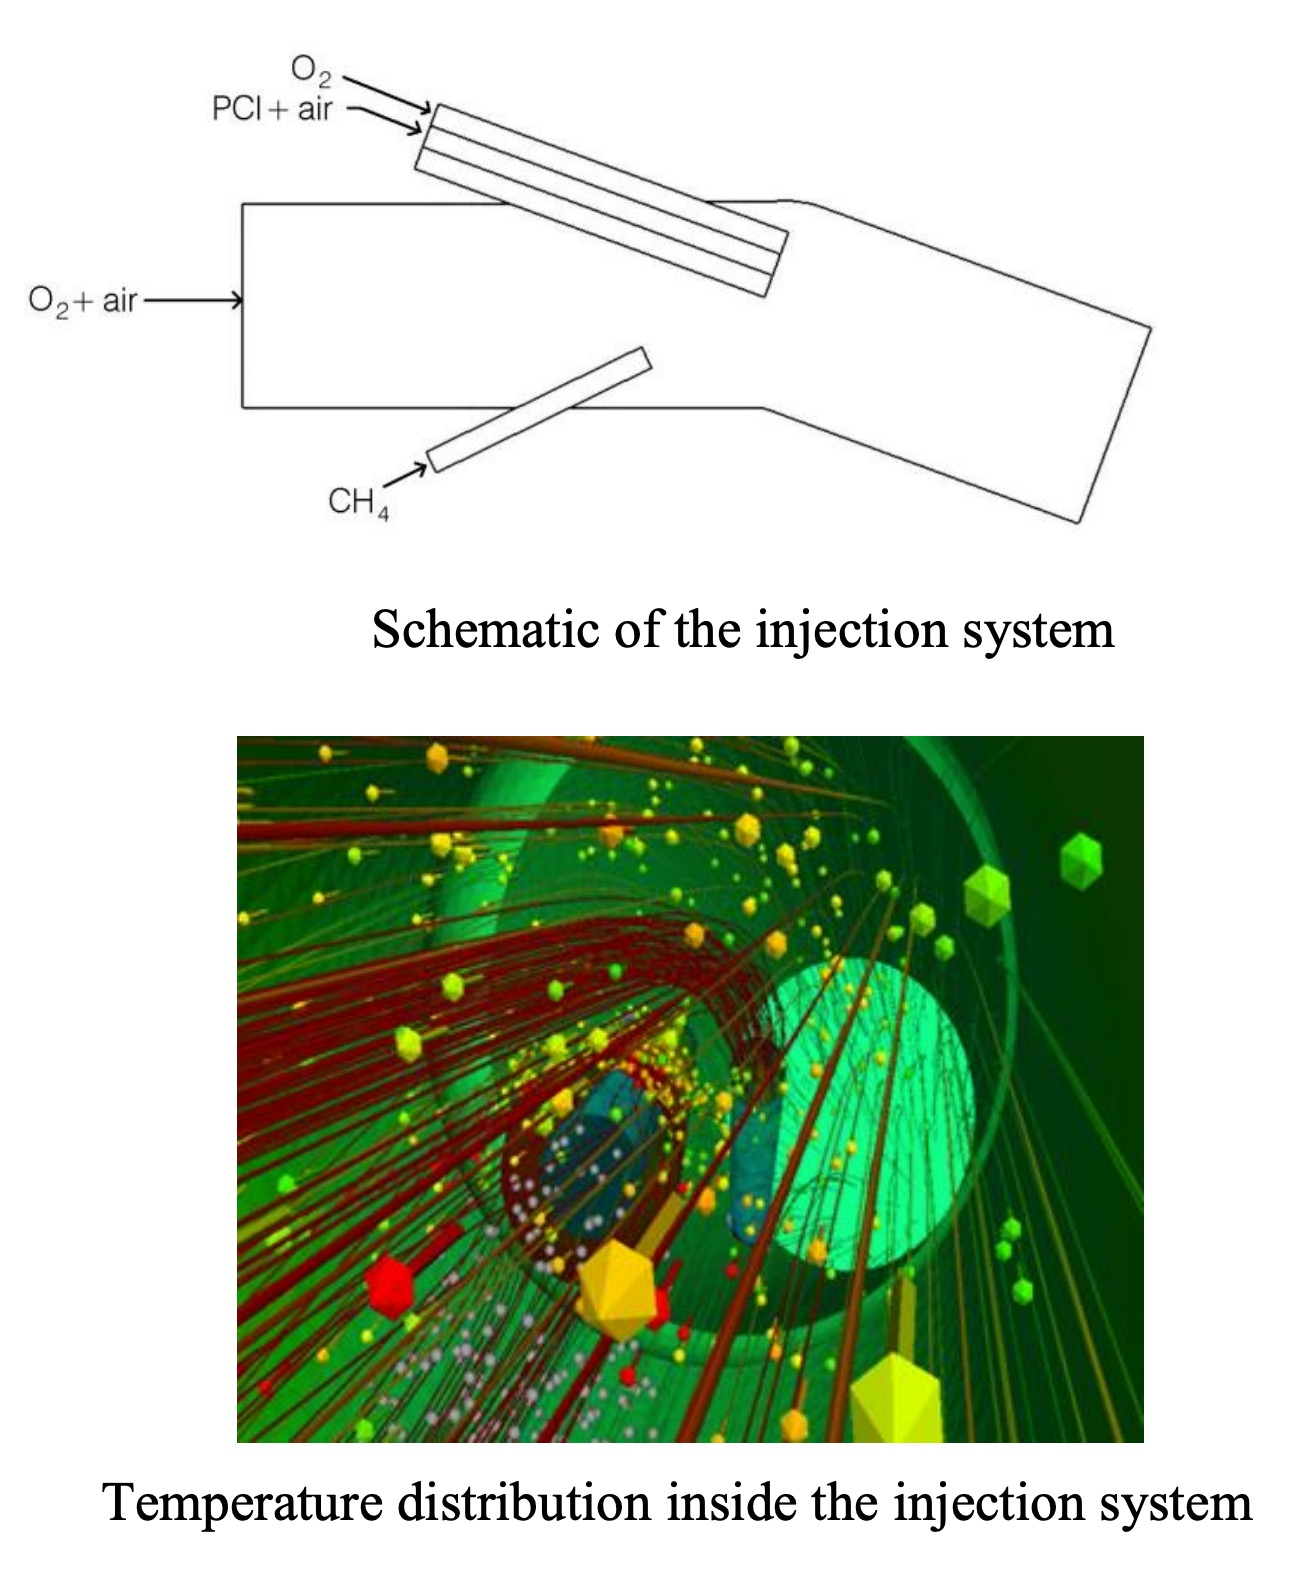
\includegraphics[width=.8\textwidth,angle=0]{cfd-injection-system.jpg}
	\caption{CFD simulation of pulverized coal injection system.}
	\label{o:m8}
\end{figure}

Effects of operating parameters such as blast temperature, natural gas flow rate, oxygen enrichment, and PCI carrier air rate were further investigated. Results form the simulation informed further realization to stop cold oxygen flow incection through the oxy-coal co-axial lance. The outcome was significant downtime avoidance due to fewer failures of~penstock and fuel lances. This process change realized a coke savings of 15 lbs/NT hot metal that resulted in a yearly potential cost avoidance of 8.5 million US dollars at full production.

Another very interesting project conducted at CIVS involved development of comprehensive package of modules for simulating multiple processes in blast furnace. 
3D CFD model shown in Fig. \ref{o:m6} has been developed by \citet{Zheng2014} specifically for~simulating the blast furnace hearth. The campaign life of a blast furnace is highly dependent on residual thickness of refractory lining in the hearth. The progress of hearth lining erosion is greatly affected by hot metal flow patterns and heat transfer in refractory under different operating conditions. CFD model incorporates both the hot metal flow and conjugate heat transfer through the refractories. They achieved consistency of results between measured and calculated refractory temperature profiles, as the model has been extensively validated using measurement data from industry blast furnace. The virtual reality (VR) visualization technology has been used to analyze the velocity and temperature distributions and wear patterns of different furnaces and operating conditions. This interactive 3D visualization is shown in Fig. \ref{o:m7}. Based on the results, it was possible to predict the inner profile of hearth and provide guidance to protecting the blast furnace hearth.

\begin{figure}[h!]
	\centering
	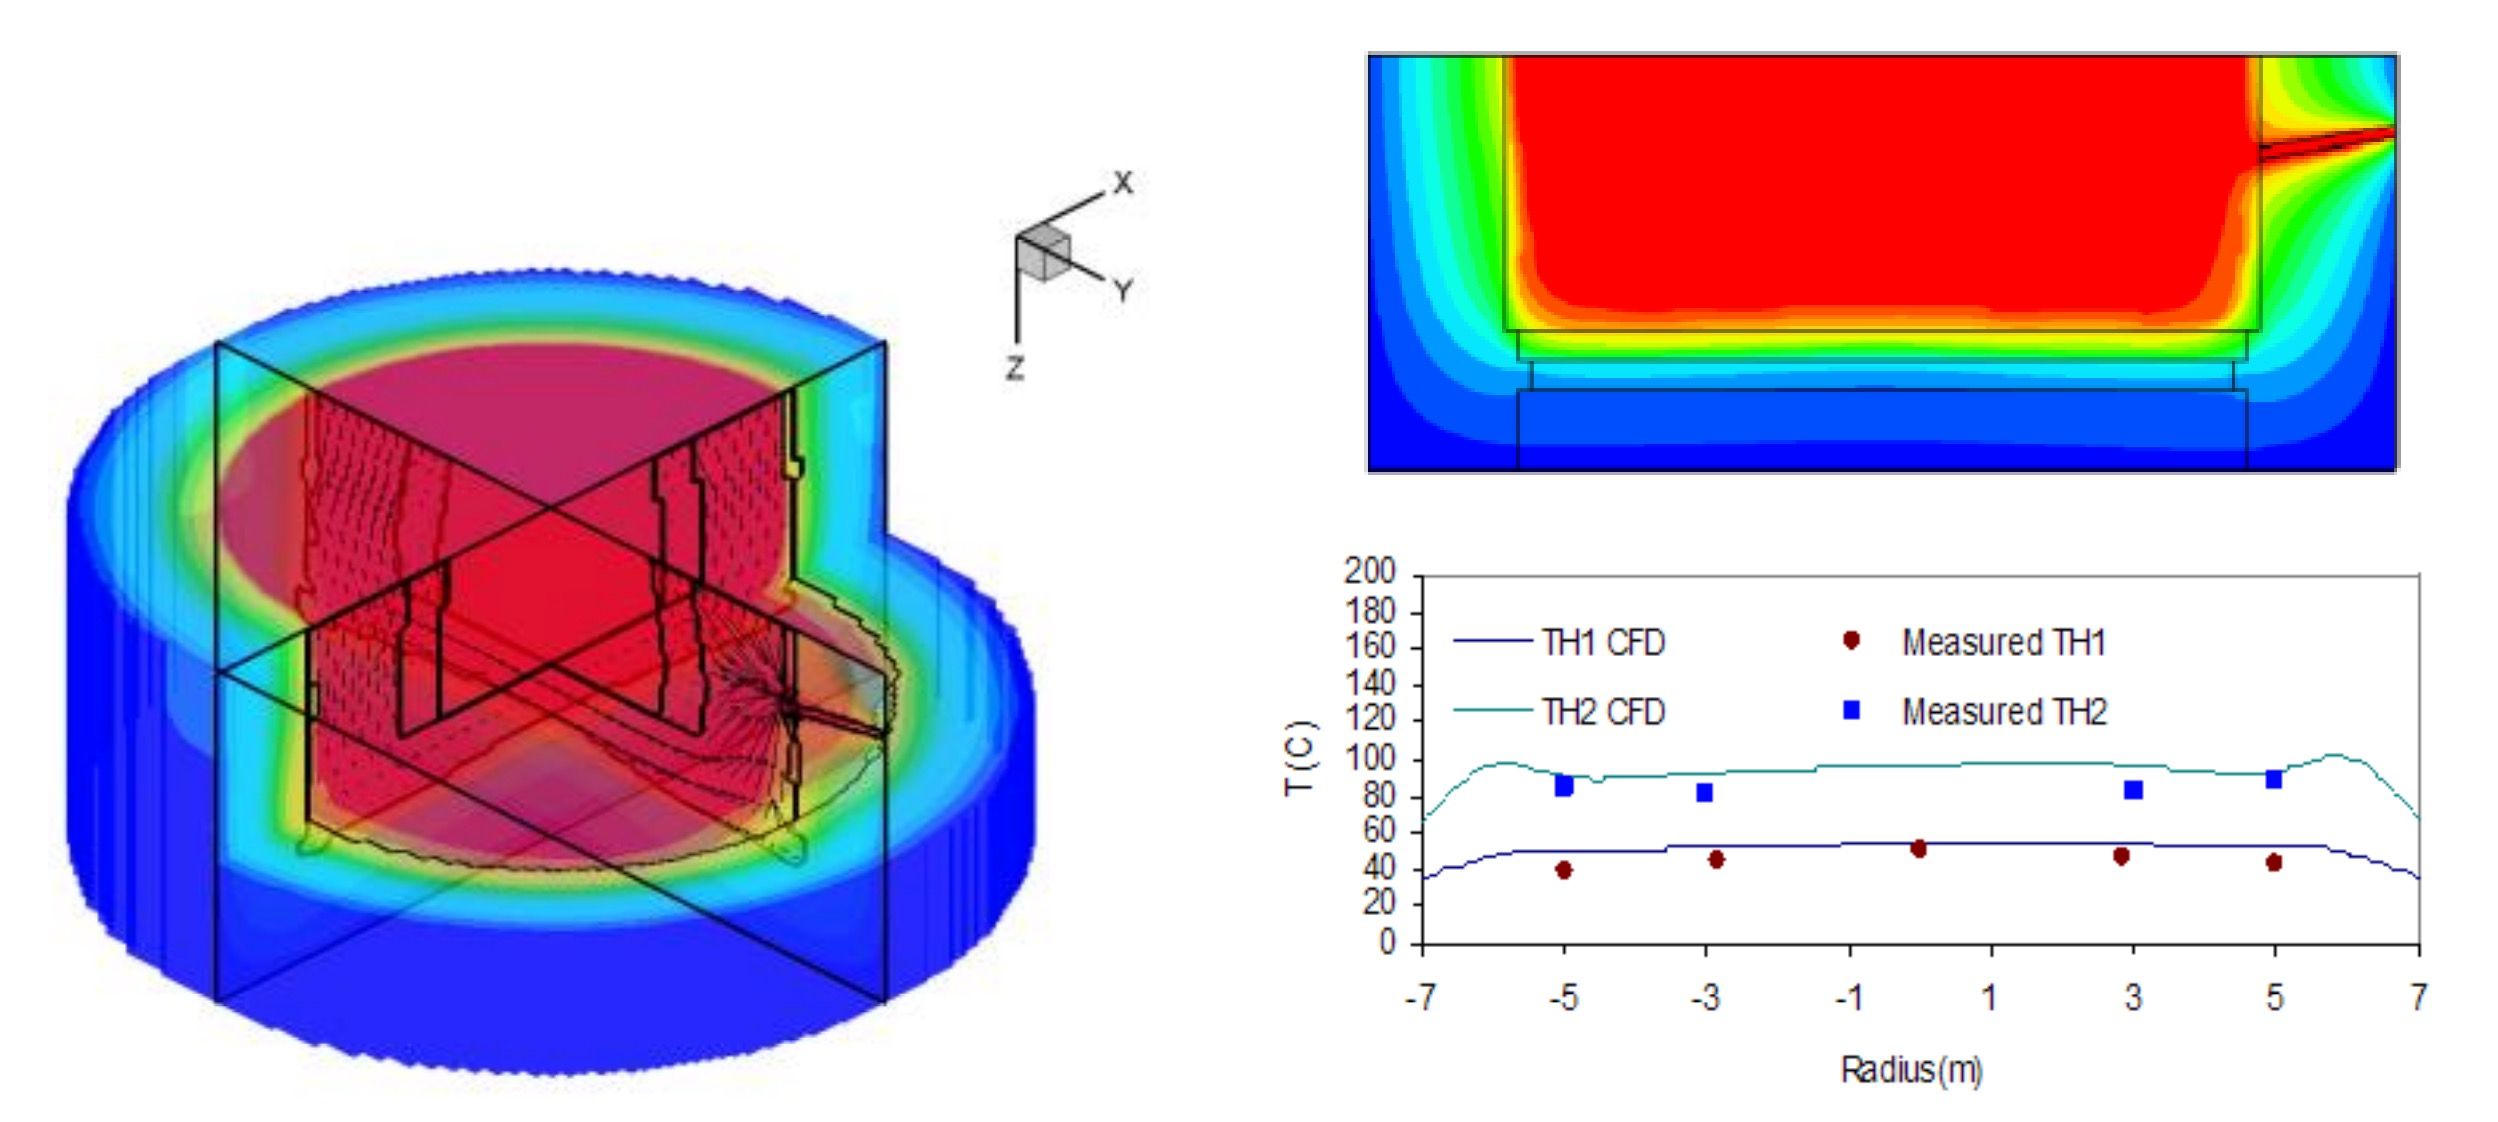
\includegraphics[width=.8\textwidth,angle=0]{blast-furnace-erosion-cfd.jpg}
	\caption{CFD model for simulation of temperature distribution in blast furnace hearth.}
	\label{o:m6}
\end{figure}

\begin{figure}[h!]
	\centering
	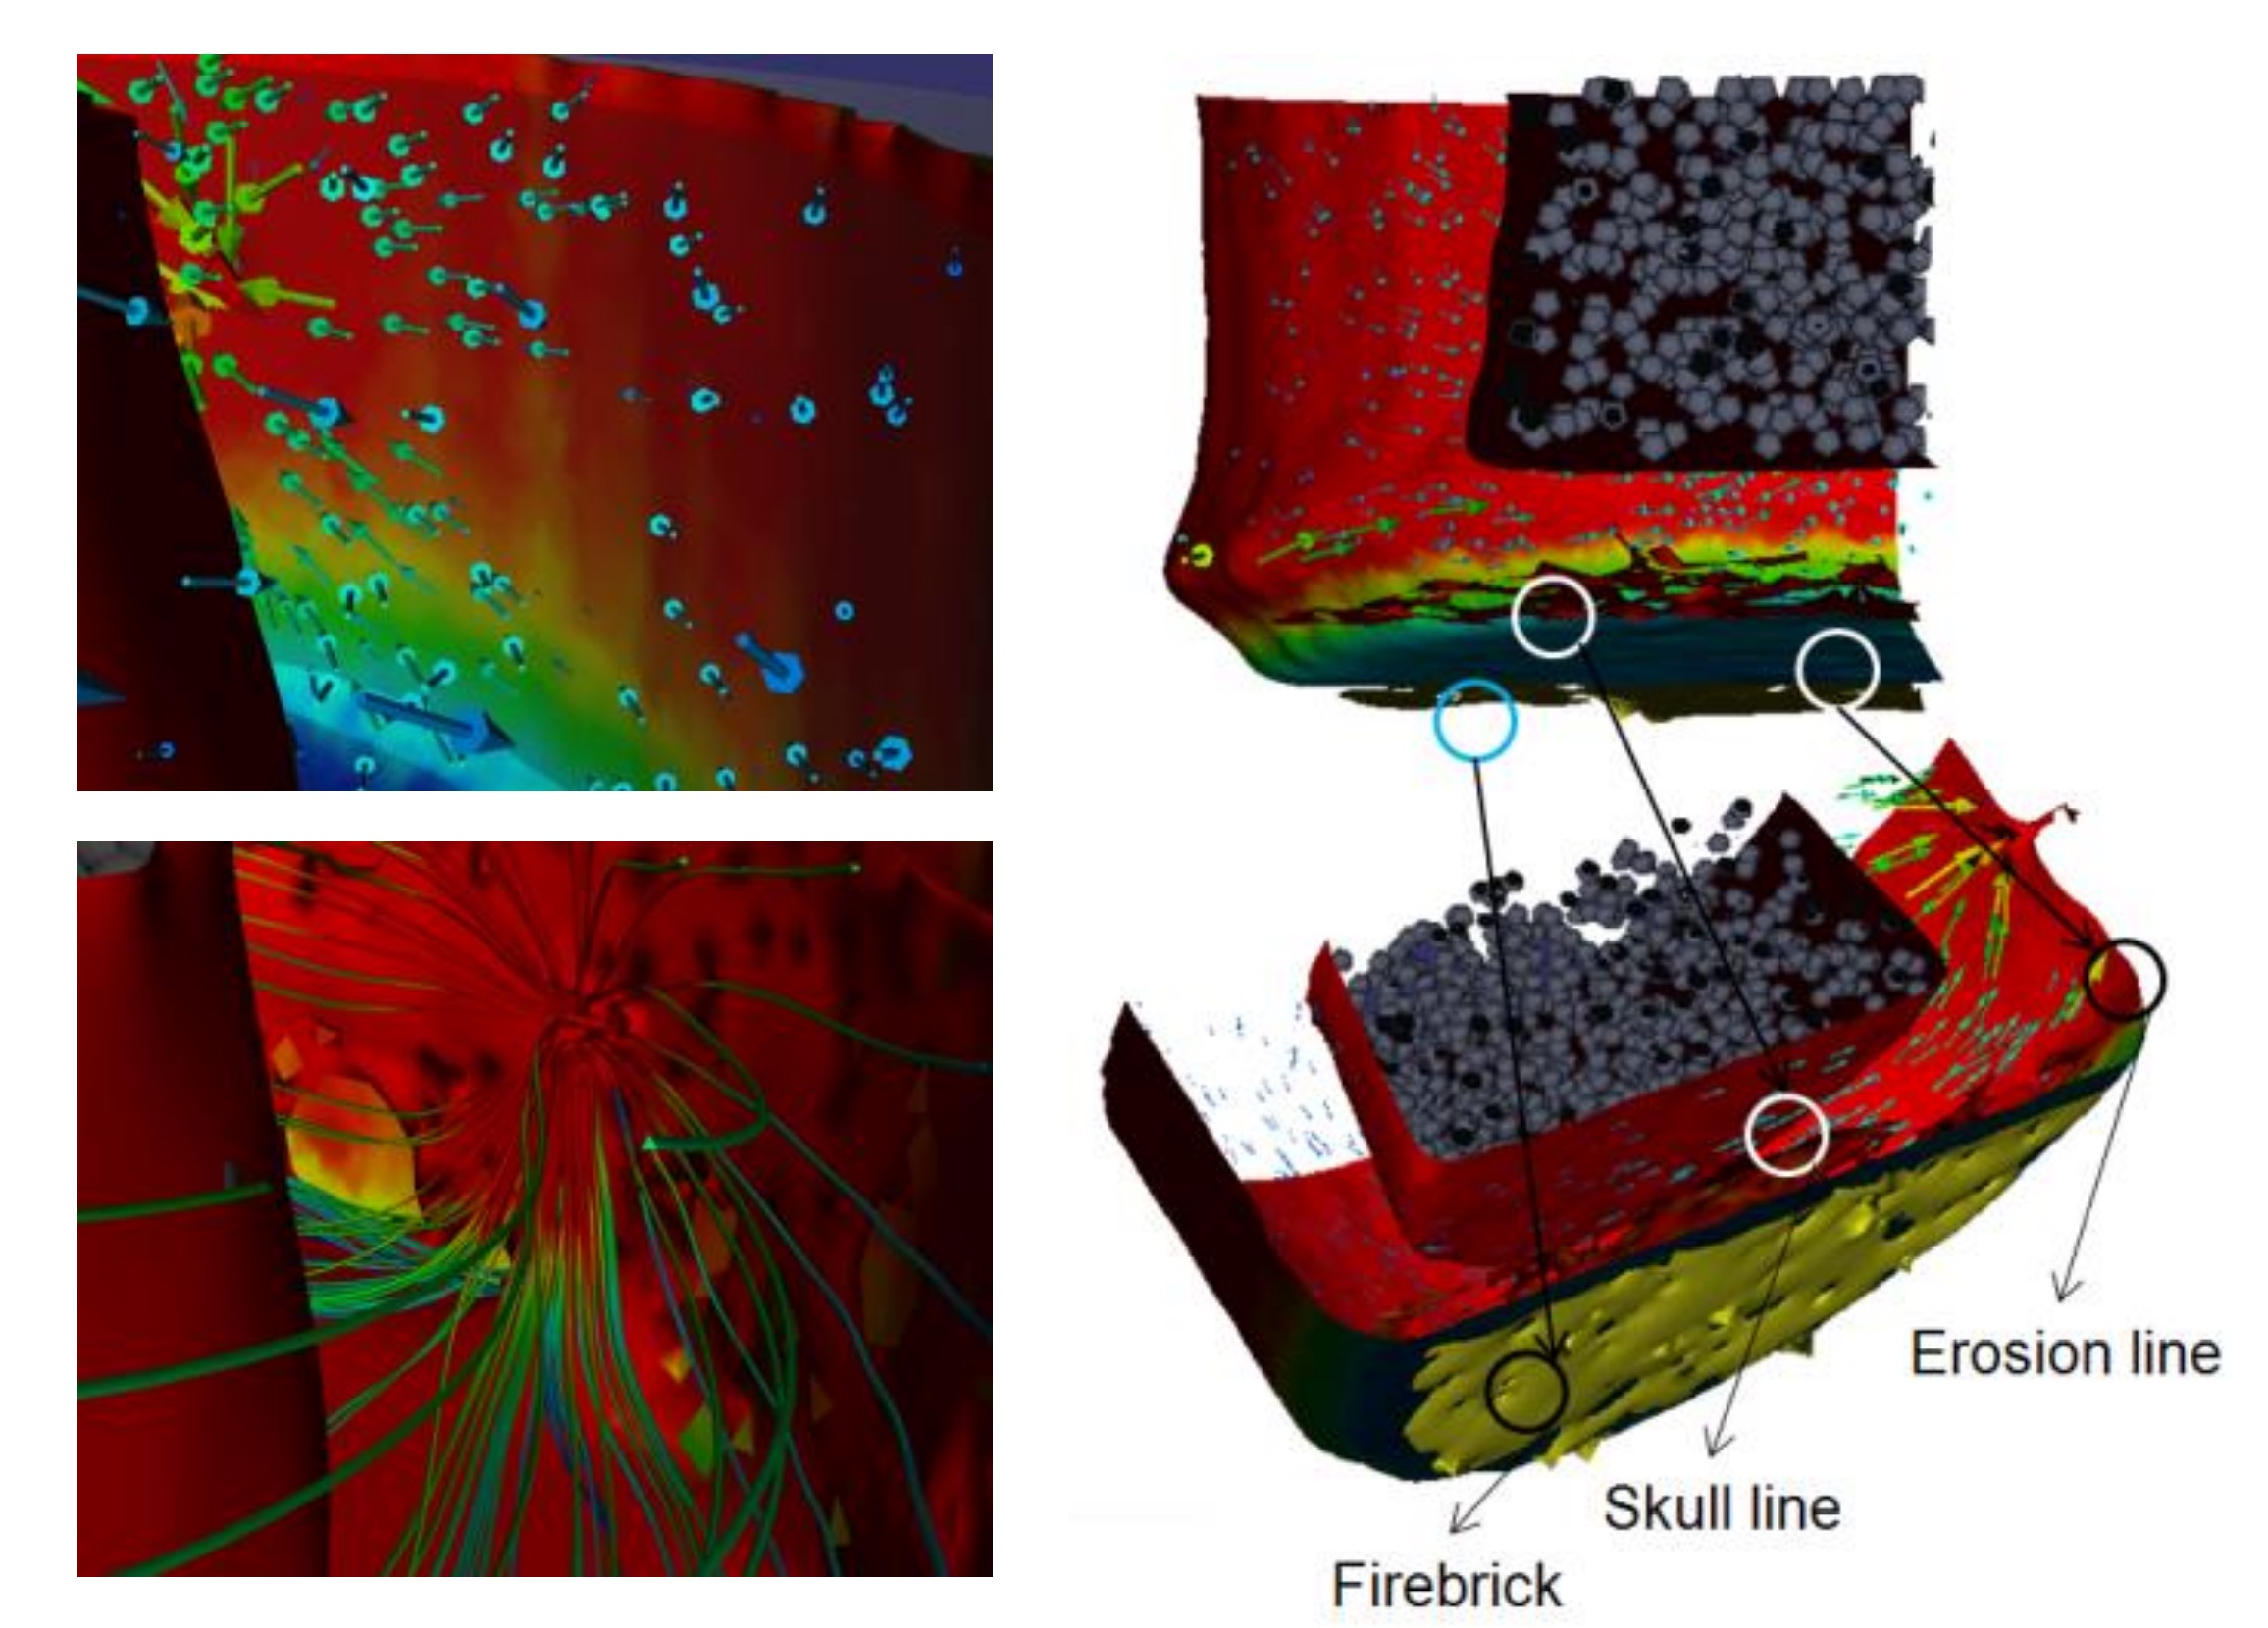
\includegraphics[width=.8\textwidth,angle=0]{blast-furnace-erosion-vr.jpg}
	\caption{3D visualization of CFD results using CAVE-based VR system.}
	\label{o:m7}
\end{figure}

Part of the project is also complex set of numerical simulations of various processes in~blast furnace combined into interactive and immersive 3D models viewable through VR headsets or explorable in CAVE systems. Fig. \ref{o:m9} describes some of the simulation packages and Fig. \ref{o:m10} shows gas and burden distribution visualization of CFD simulation inside blast furnace shaft.

\begin{figure}
	\centering
	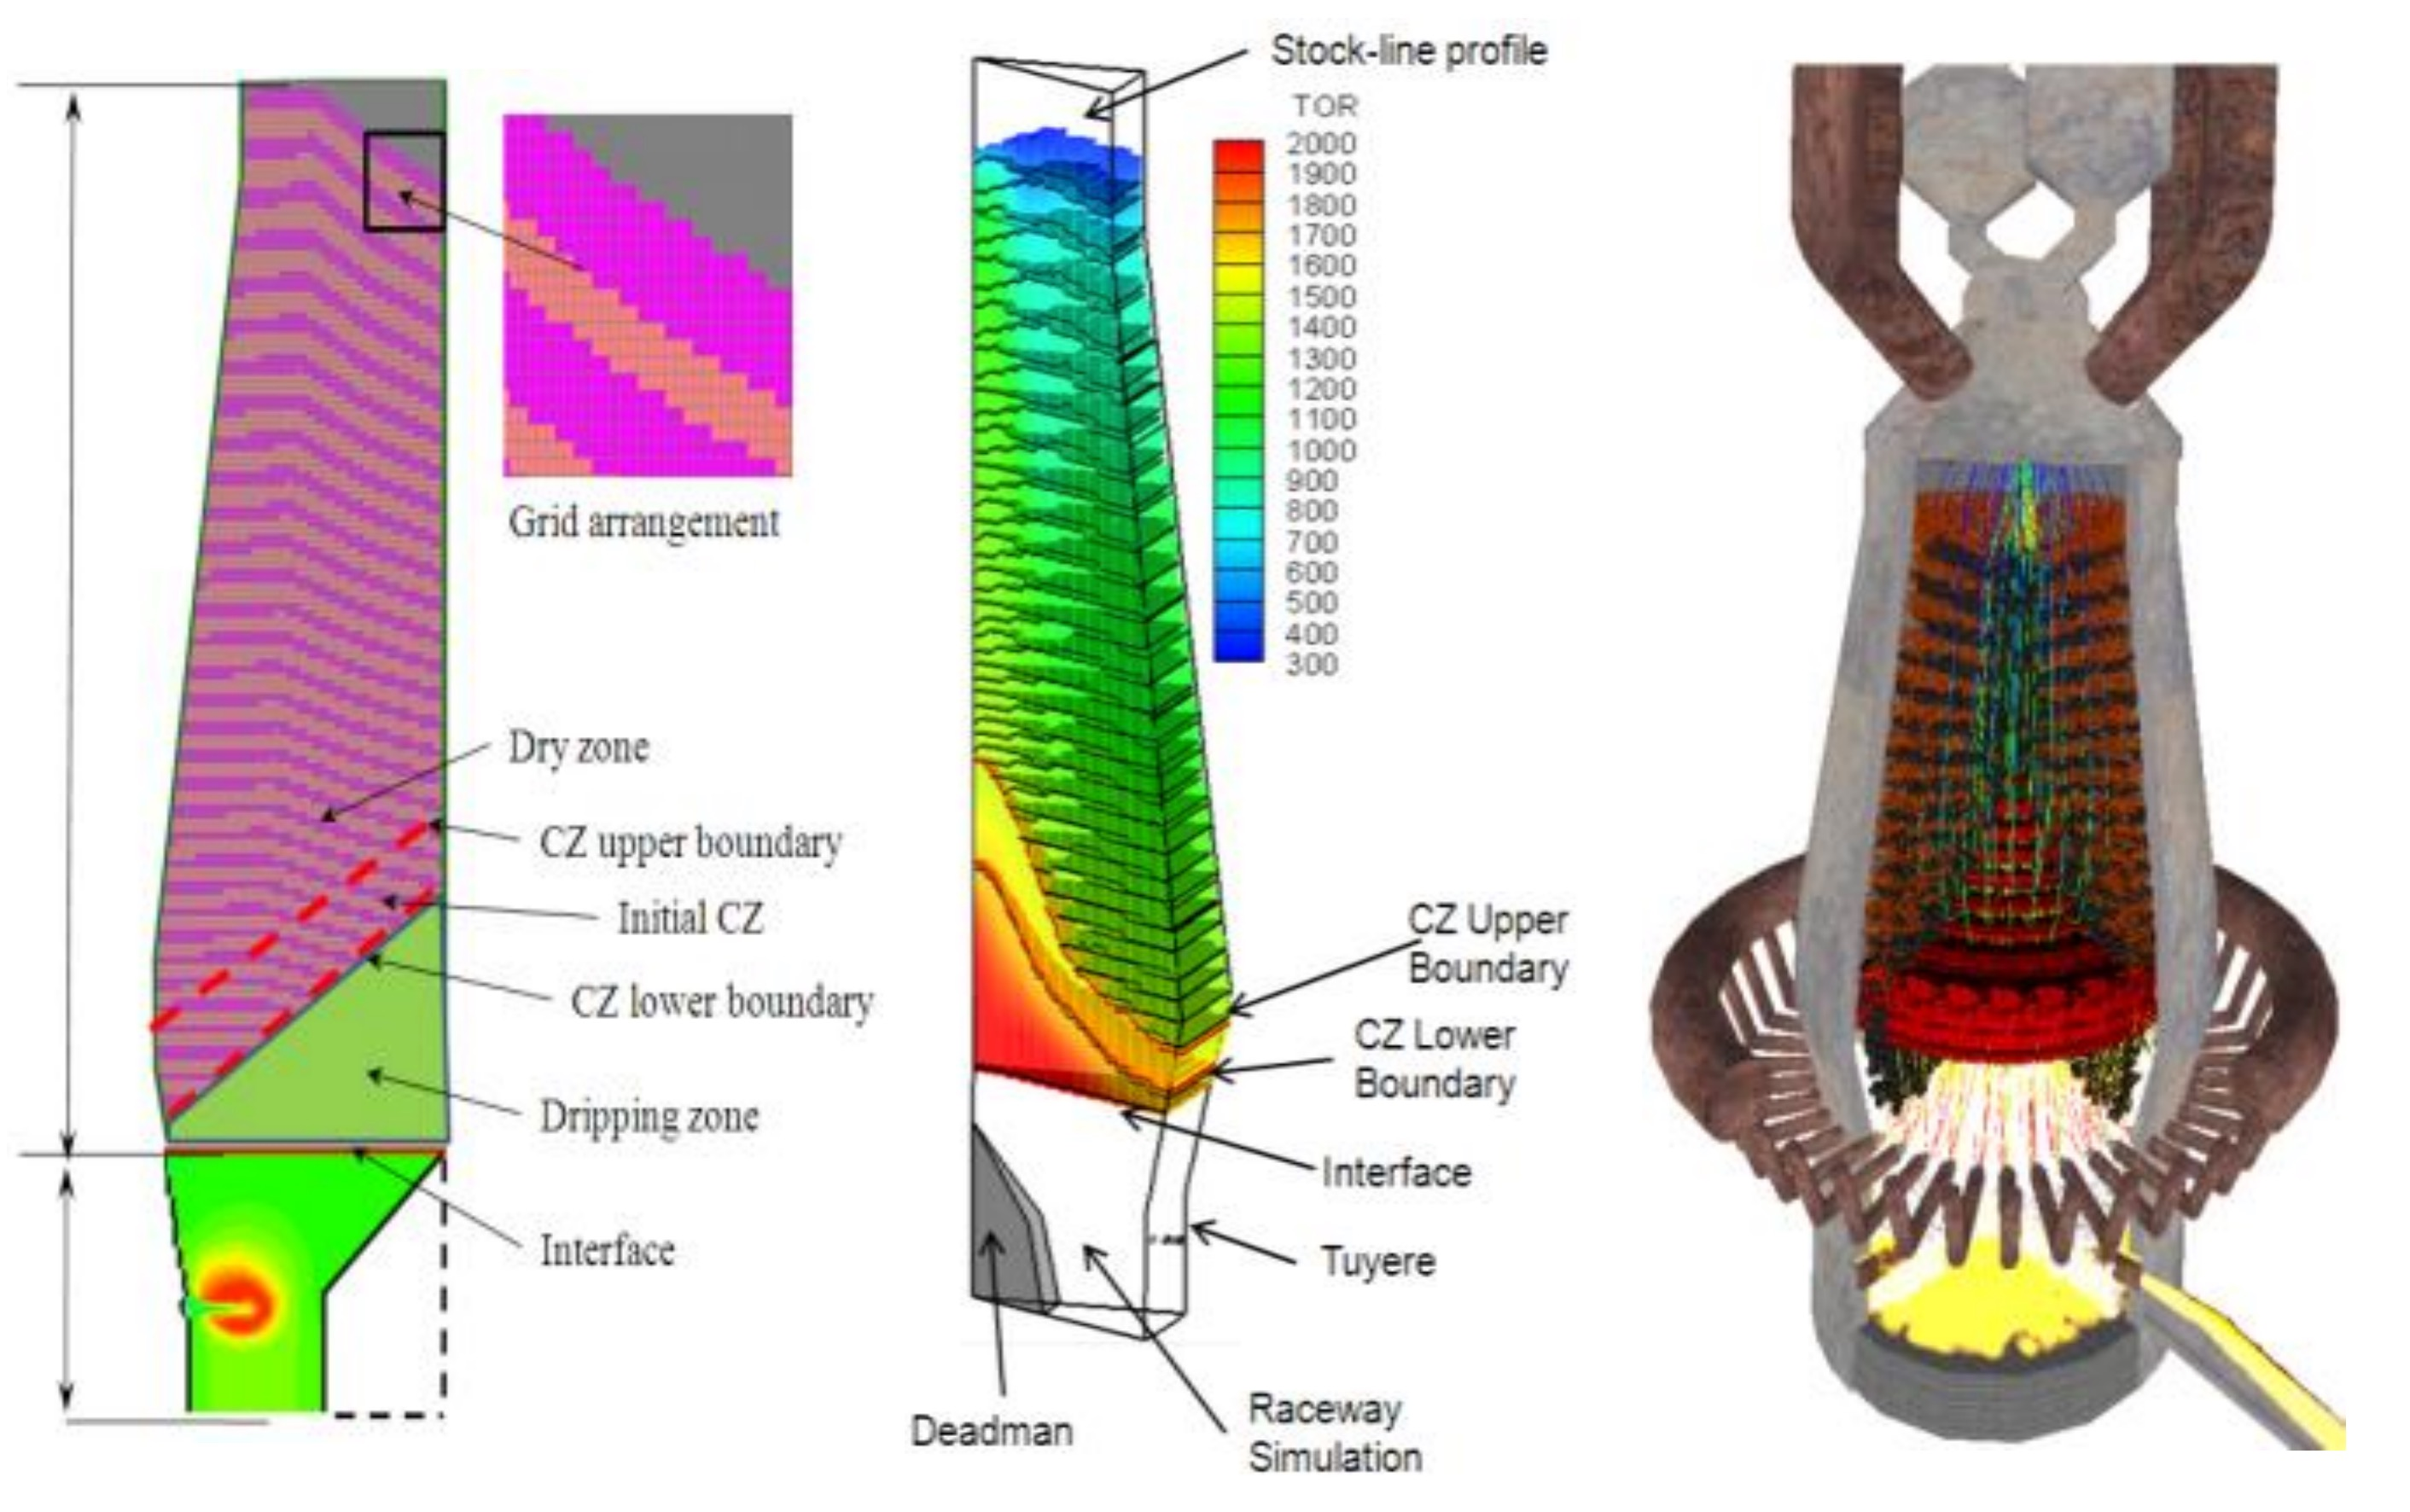
\includegraphics[width=1\textwidth,angle=0]{blast-furnace-simulation-and-viz.jpg}
	\caption{Blast furnace simulation and visualization}
	\label{o:m9}
\end{figure}

\begin{figure}
	\centering
	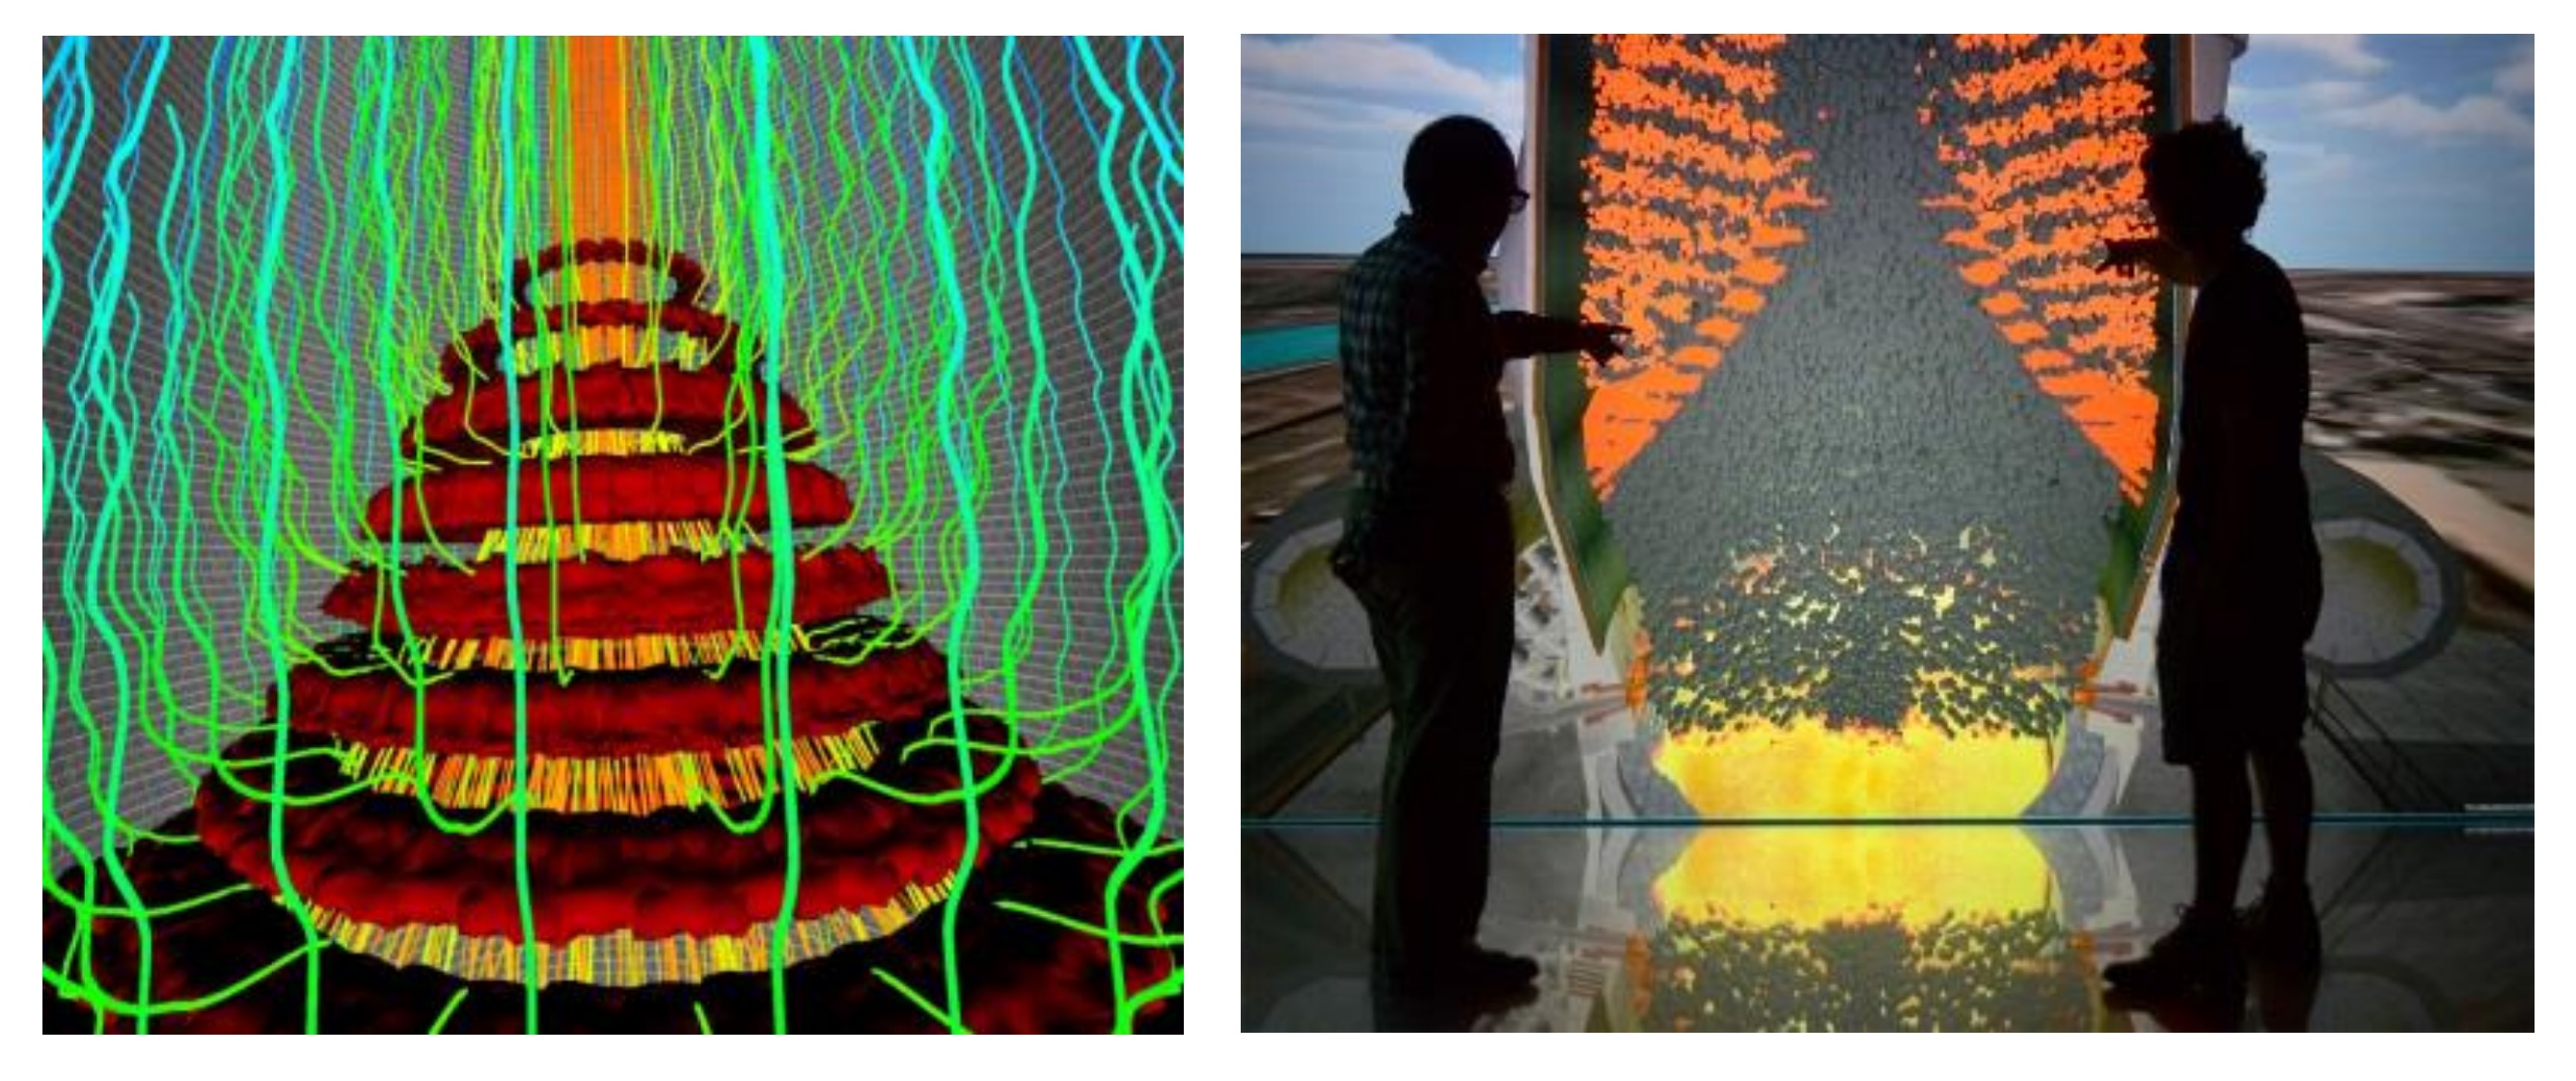
\includegraphics[width=1\textwidth,angle=0]{blast-furnace-gas-burden.jpg}
	\caption{3D visualization of gas and burden distribution inside blast furnace shaft}
	\label{o:m10}
\end{figure}

\newpage
\section{Objectives and methodology of the dissertation}
\label{section:3}
This dissertation thesis deals with design and implementation of modern methods in process control. Since I have been consulting and working professionally with virtual reality and at the Institute of Control and Informatization of Production Processes, where significant work has been done in steelmaking field with focus on basic oxygen process (LD/BOF), I've decided to focus my attention to using VR technology and interactive 3D graphics for modeling, simulating and optimizing the LD/BOF process. I've been in~close contact with other researchers that have hands on experience with research in this area \citep{Kacur2019,Sprava2018} which provides me with the much of~the needed consultations, further contact with steelmaking industry companies in Košice and~central European region, and~data gathered from numerous studies.

As research studies and projects implemented at CVIS shown, new trends like high-resolution 3D simulation and VR technology can be largely helpful in optimizing metallurgical processes. Immersive VR simulations of blast furnace presented in previous section clearly shown potential of these technologies and delivered significant economical impact. As vast majority of steel manufactured in the world is produced using the LD/BOF process, similar approaches should be considered and tried as for the blast furnace mentioned above in section \ref{subsection:2.4}. 

Main objectives of this dissertation are as follows:

\begin{enumerate}
\item{Static, high-quality 3D representation of LD converter will be modeled, with walls and inner parts each modeled separately, so the 3D model is modular enough for further work that involves composing static and dynamic parts together. Work on~this phase was already started, with design and 3D modeling of basic oxygen furnace (LD converter) based on models from steeluniversity.org in open-source, 3D modeling software, Blender. In the meantime, discussions about possible collaboration with SteelUniversity has been initiated with the goal of taking advantage of already existing static 3D models like the one shown in Fig. \ref{o:3.1}.

\begin{figure}[ht!]
	\centering
	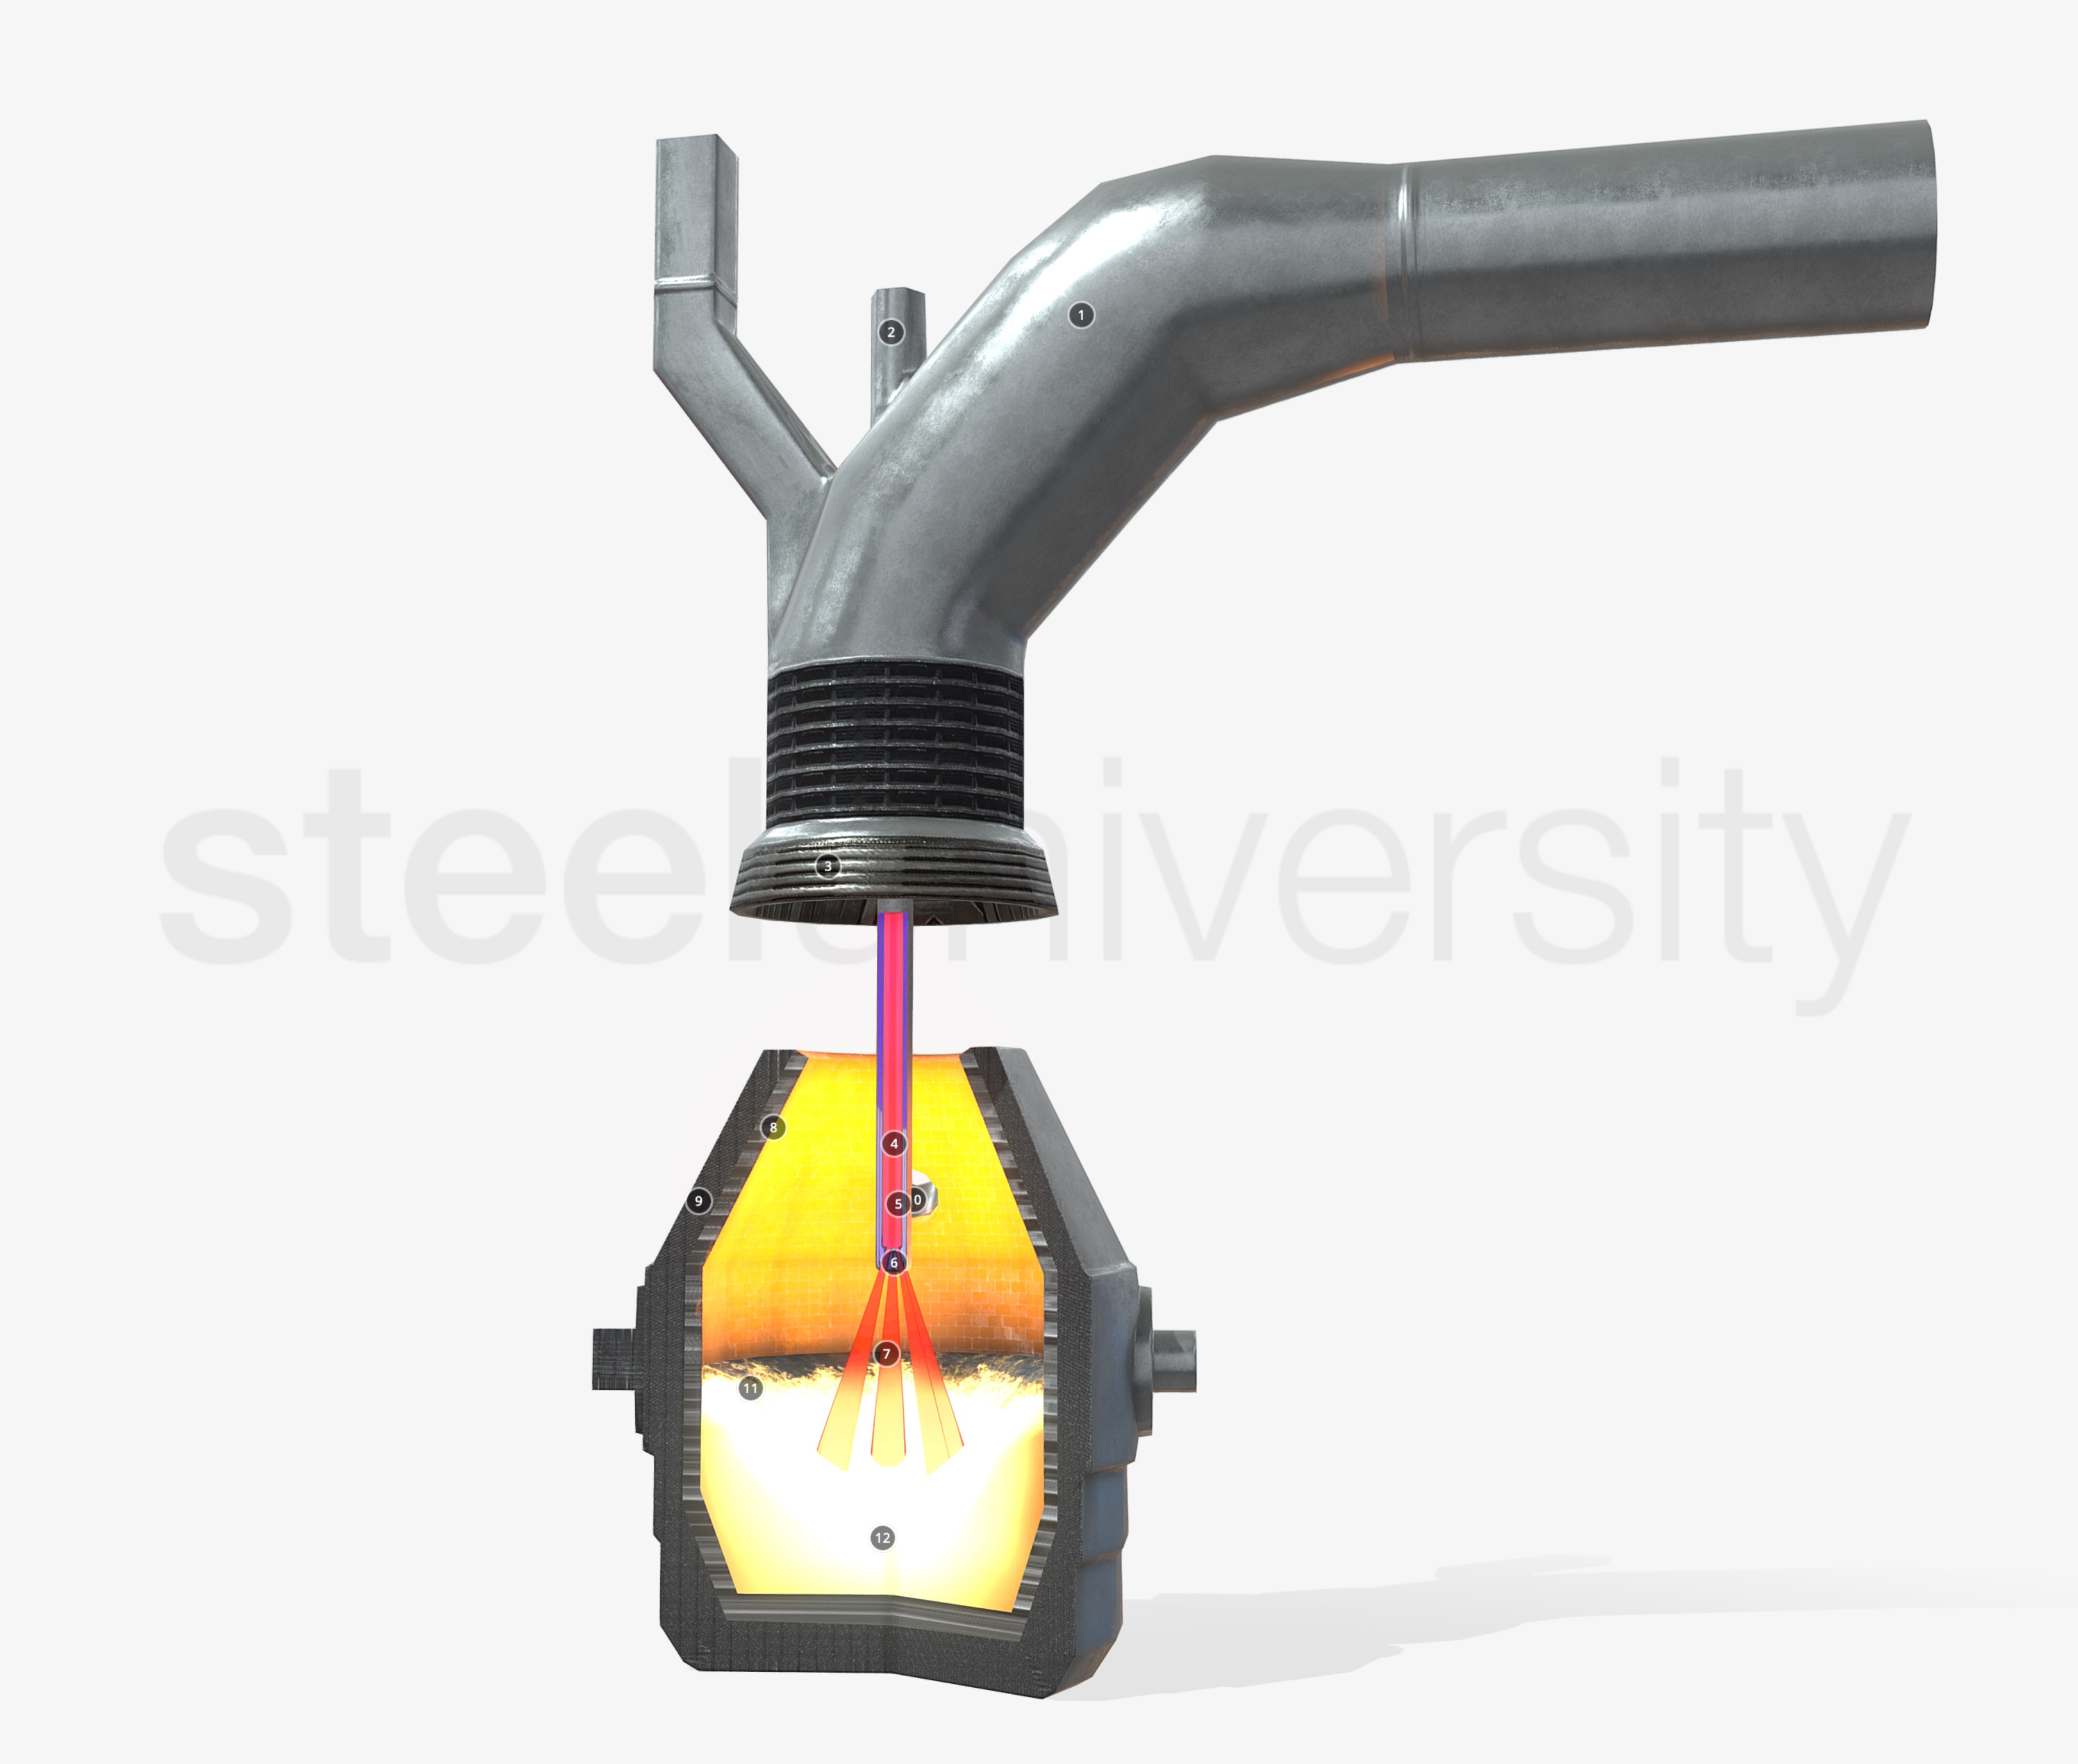
\includegraphics[width=.74\textwidth,angle=0]{bof-static-model.jpg}
	\caption{Annotated model of LD converter with information about each part that can be displayed by clicking on the numbers (created by steeluniversity.org and hosted on Sketchfab). It has been created for educational purposes.}
	\label{o:3.1}
\end{figure}

}
\item{3D simulations of chemical and thermodynamical processes in basic oxygen steelmaking will be created with use of computational fluid dynamics (CFD) methods. CFD software like ANSYS, SimScale and OpenFOAM will be analyzed and most suitable one picked for creation of aforementioned simulations. Special attention will be placed on interactivity features and how visual exploration of final simulations can be achieved. Interactivity of 3D models and manipulation of simulation time scales is of great importance.}
\item{Immersive environment in virtual reality will be designed and implemented in Unity and Unreal Engine software. It will be designed to be used in conjunction with off-the-shelf, commercial, six-degrees-of-freedom (6DoF) VR headsets, hand controllers and hand trackers. It will include combination of static 3D models of LD converter (in different variations e.g. with varied opacity of the walls or bisected) with dynamic, interactive inner part consisting of 3D multi-phase CFD model simulating chemical and thermodynamical processes. These will be viewable separately or in combination according to user's preference. Impact of provided immersiveness to deepening of the understanding of various known processes and searching for hidden issues presenting themselves through simulations in this setting will be studied and analyzed.}
\item{Novel interactive 3D graphical interfaces for multi-phase virtual reality simulation will be designed and implemented. Hand and finger tracking will play important role in design of these interfaces. Users should be able to step into the live 3D simulation, use their hand as a pointer to get immediate feedback and information like slag temperature by pointing the laser ray from their hand at any point on~the~top of~the~slag or~manipulate the time scales of the simulation by moving the slider on~a~timeline (inspired by time-travel debugging techniques utilized in game development and novel programming tools).}
\item{Possible by-product after finalization of previous objectives is the educational use of tools that will be created as a part of this dissertation. Relatively small tweaking of the software created would be needed to build a separate tool for training purposes of future converter operators, or in a more general way as a educative tool at~technical universities.}
\end{enumerate}

